\section{Task 2}\label{sec:task2}

The goal of the second task is to implement a tool able to describe the relationship between ensembles of a PED, from global and local points of view. Relationships between different ensembles will be evaluated thanks to PED features. The input are files, each containing ensemble features, computed during Task 1.

\subsection{Ensembles features}
For each ensemble, PED features are extracted from the previously computed models features. In details, the obtained features are the following:

\begin{itemize}
\item[-] \emph{Radius of gyration} (RG) is retrieved for each model. It may happen that an ensemble contains a lower number of conformations with respect to the others. To avoid alignment problems, zero-padding is performed.
\item[-] \emph{SS entropy} is calculated for each position across ensemble's conformations, exploiting its probabilistic definition.
\item[-] \emph{Median ASA} is computed for each position across ensemble's conformations.
\item[-] \emph{Median RMSD} is computed using roto-translation matrices across ensemble's conformations.
\item[-] \emph{Median distance matrix} is computed by calculating median distance for each pair of equivalent positions across ensemble's conformations.
\item[-] \emph{Standard deviation distance matrix} is computed calculating standard deviation distance for each pair of equivalent positions across ensemble's conformations.
\end{itemize}

\subsection{Global metric}
The global metric aims to provide an accurate measure of dissimilarity between ensemble pairs represented with their features, building an evaluation that takes into account the different nature of the features evaluated. Given two ensemble features vectors, the sum of the following partial distances is returned:
\begin{itemize}
\item[-] Absolute difference of RG mean values extracted from each feature vector, after zero-padding removal.
\item[-] Chebyshev distance\footnote{\textbf{Chebyshev distance} : a.k.a maximum metric, is a metric defined on a vector space where the distance between two vectors is the greatest of their differences along any coordinate dimension.} calculated between entropies vectors.
\item[-] Euclidean distance calculated between median ASA vectors.
\item[-] Euclidean distance calculated between median RMSD vectors.
\item[-] Cosine distance calculated between median distance vectors.
\end{itemize}

Standard deviation distance matrix has not been taken into consideration for the global evaluation, since it is a kind of variability measure for each residue and that does not provide useful information from a global point of view.

Results of global distances application inside PEDs are provided through an \emph{heatmap} which shows distances between each pair of ensembles thanks to a color-map and a \emph{dendrogram} which exploits a linkage matrix to apply a \emph{complete} linkage approach.
Figures \ref{heatmap} and \ref{dendrogram} show respectively distances and similarity relationships between analyzed ensembles. From the heatmap analysis, it is possible to notice that ensembles 002 and 003 are the closest ones, whereas 001 and 002 are the furthest ones. In general, all ensembles seem to be evenly spaced from each other. In addition, a more precise understanding of the spatial distribution can be inferred from the dendrogram, in which two clearly visible sub-clusters are revealed, in detail the first containing 002, 003 and 004 and the second 001 and 005.

\begin{figure}[H]
    \centering
	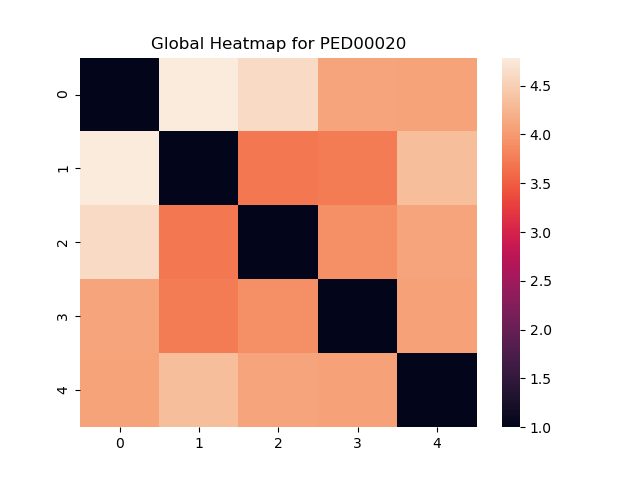
\includegraphics[width=\textwidth]{PED00020_heatmap.png}
	\caption{Heatmap of all the ensembles.}
	\label{heatmap}
\end{figure}
\begin{figure}[H]
    \centering
	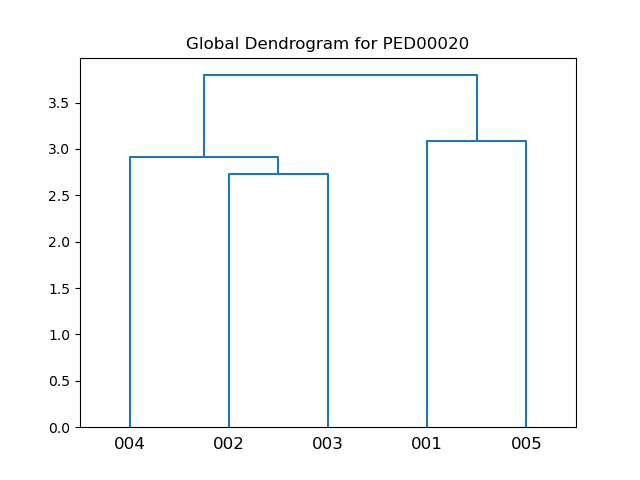
\includegraphics[width=\textwidth]{PED00020_dendrogram.png}
	\caption{Dendrogram of all the ensembles.}
	\label{dendrogram}
\end{figure}


\subsection{Local metric}
The local metric evaluates the ensembles' features variability for each residue.
The i-th residue variability is calculated considering a window of 19 (9 before and 9 after) residues around the current one. After extracting the features vectors of those residues, a variability score is calculated independently for each type of feature as follows:

\begin{itemize}
\item[-] Mean window value of the standard deviations calculated among conformational entropies for each residue.
\item[-] Mean window value of the standard deviations calculated among conformational ASA for each residue.
\item[-] Mean window value of the standard deviations calculated among conformational RMSD values for each residue.
\item[-] Trimmed mean\footnote{\textbf{Trimmed mean}: used to to avoid outliers influence.} window value of the standard deviation of conformations distances for each residue.
\end{itemize}

Each variability score is then used to calculate the residue mean variability value. In figure \ref{plot} each residue variability in terms of ensembles' features is shown.

\begin{figure}[H]
    \centering
	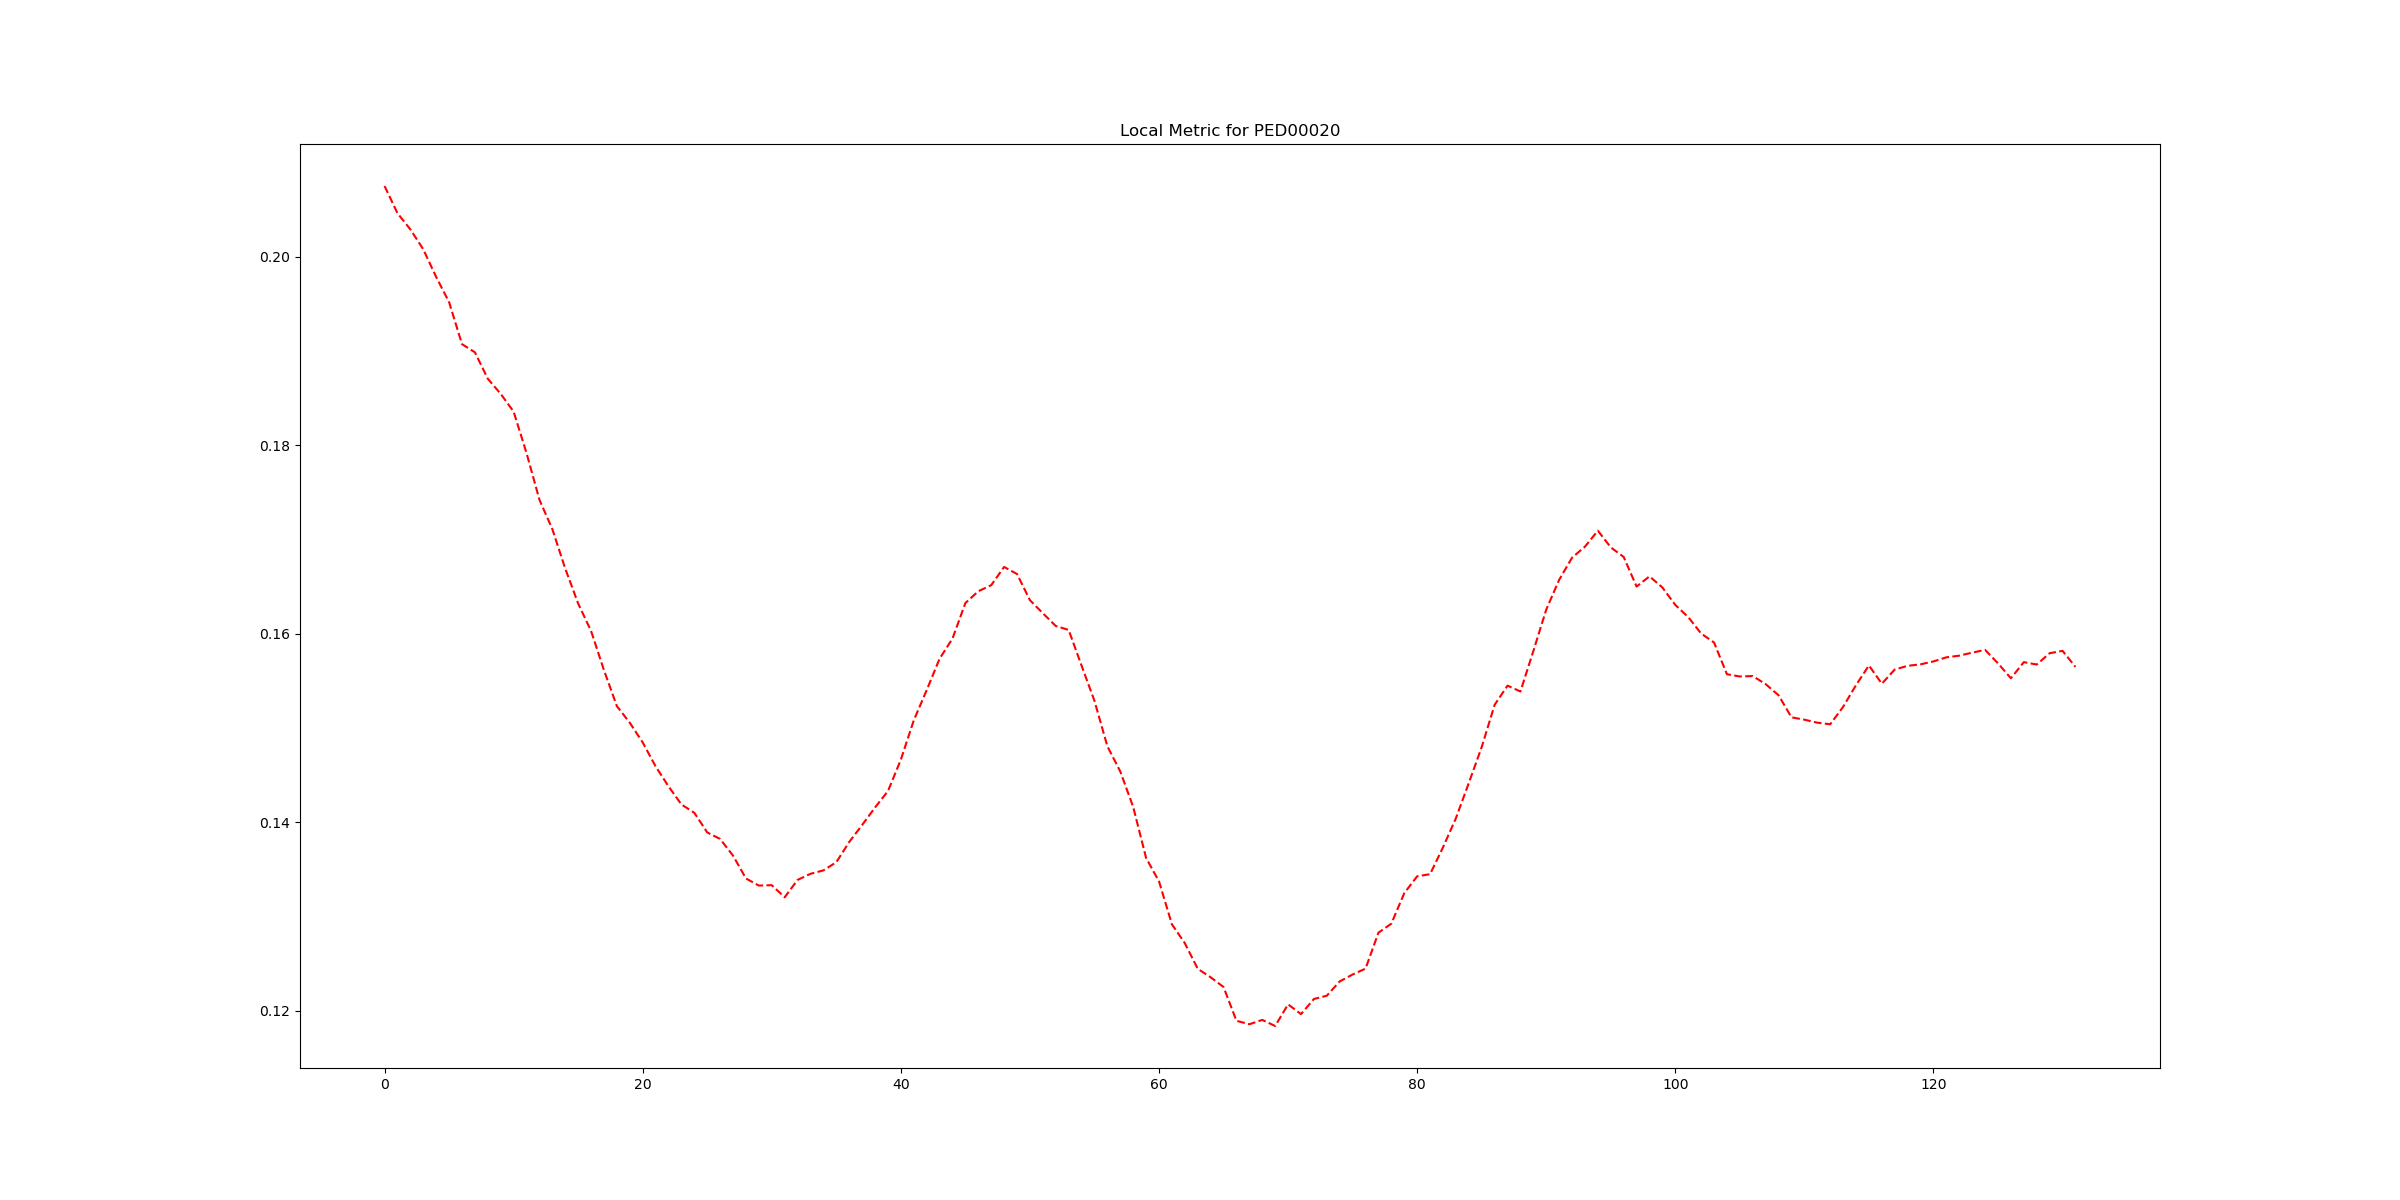
\includegraphics[width=\textwidth]{PED00020_local.png}
	\caption{Plot of local score.}
	\label{plot}
\end{figure}

Since the graph shows an average value among all the ensembles, it is not possible to make an exhaustive comparison between its behaviour and the structure variability in Pymol images, even if it allows to infer general considerations about disordered content. The measles virus nucleoprotein seems to be quite disordered: in particular, all the ensembles share a central high variability region (that could be associated with one of the local maxima), whereas some of them have another variable region in one of the extremities. Due to the smaller available window on the trailing parts, correspondent scores could be less trusted with respect to the central parts of the protein in which, except ensemble 005, is located the most stable region.

The previous analysis can lead to these intuitions but the final protein study should be performed with additional information. Since the protein has the stable region in its center, these residues might be in charge of some functional properties. On the contrary, the most variable regions could not be useful from a functional point of view or could allow the protein to respond to stimuli in different ways.